% Created 2021-10-04 Mon 10:19
% Intended LaTeX compiler: pdflatex
\documentclass[11pt]{article}
\usepackage[utf8]{inputenc}
\usepackage{lmodern}
\usepackage[T1]{fontenc}
\usepackage[top=1in, bottom=1.in, left=1in, right=1in]{geometry}
\usepackage{graphicx}
\usepackage{longtable}
\usepackage{float}
\usepackage{wrapfig}
\usepackage{rotating}
\usepackage[normalem]{ulem}
\usepackage{amsmath}
\usepackage{textcomp}
\usepackage{marvosym}
\usepackage{wasysym}
\usepackage{amssymb}
\usepackage{amsmath}
\usepackage[theorems, skins]{tcolorbox}
\usepackage[version=3]{mhchem}
\usepackage[numbers,super,sort&compress]{natbib}
\usepackage{natmove}
\usepackage{url}
\usepackage[cache=false]{minted}
\usepackage[strings]{underscore}
\usepackage[linktocpage,pdfstartview=FitH,colorlinks,
linkcolor=blue,anchorcolor=blue,
citecolor=blue,filecolor=blue,menucolor=blue,urlcolor=blue]{hyperref}
\usepackage{attachfile}
\usepackage{setspace}
\usepackage{geometry}
\geometry{margin=1.0in}
\usepackage{outline}
\usepackage{amsmath}
\usepackage{graphicx}
\usepackage{epstopdf}
\usepackage{fancyhdr}
\usepackage{hyperref}
\usepackage{siunitx}
\usepackage[labelfont=bf]{caption}
\setlength{\headheight}{15.2pt}
\def\dbar{{\mathchar'26\mkern-12mu d}}
\pagestyle{fancy}
\fancyhf{}
\renewcommand{\headrulewidth}{0.5pt}
\renewcommand{\footrulewidth}{0.5pt}
\lfoot{\today}
\cfoot{\copyright\ 2021 W.\ F.\ Schneider}
\rfoot{\thepage}
\lhead{\em{Advanced Chemical Reaction Engineering}}
\rhead{ND CBE 60546}
\setcounter{secnumdepth}{3}
\author{William F. Schneider}
\date{\today}
\title{CBE 60546 Outline}
\begin{document}

\begin{OPTIONS}
\end{OPTIONS}
\section{Lecture 0: Intro to Reaction Engineering}
\label{sec:org2246e86}
\begin{enumerate}
\item Reaction engineering
\end{enumerate}
\begin{quote}
Understanding, modeling, designing, using, controlling, analyzing, improving anything in which chemical reactions happen.
\end{quote}
\begin{enumerate}
\item Reaction engineering applications
\begin{enumerate}
\item Traditional
\begin{enumerate}
\item Industrial chemical/petroleum processes
\item Fine chemical/pharmaceutical processes
\item Emerging, eg biorefinergy, shale gas, \url{http://cistar.us}
\end{enumerate}
\item Energy storage, batteries, fuel cells
\item Environmental systems
\begin{enumerate}
\item Atmosphere, lake, bioreactor (water purification), catalytic convertor
\end{enumerate}
\item Biological systems
\begin{enumerate}
\item Cell, organ, body
\end{enumerate}
\item Laboratory reactors - interrogate, quantify
\item Research - improved materials (catalysts), improved processes, understand limitations
\begin{enumerate}
\item Sabatier plot, \url{https://doi.org/10.1038/nchem.121}
\end{enumerate}
\end{enumerate}
\item Course structure
\begin{enumerate}
\item Quantifying chemical reactions
\begin{enumerate}
\item Stoichiometry
\item Thermodynamics - heat flow, direction, equilibrium
\item Kinetics - rates, mechanisms
\end{enumerate}
\item Physical/chemical interactions
\begin{enumerate}
\item Transport, mixing, diffusion resistance, \ldots{}
\end{enumerate}
\item Chemical reactors
\begin{enumerate}
\item Ideal 0 and 1-dimensional
\item Non-ideal
\item Non-isothermal
\item Non-steady state
\item Multiphase
\end{enumerate}
\item Chemical processes (beyond us)
\item Markets (beyond us)
\end{enumerate}
\end{enumerate}

\section{Lecture 1: Stoichiometry and reactions}
\label{sec:orga559425}
\begin{enumerate}
\item Substances
\item Amounts
\begin{enumerate}
\item mass, moles, volumes
\item flow rates
\end{enumerate}
\item compositions
\begin{enumerate}
\item amount/total amount
\end{enumerate}
\item Reactions and stoichiometric coefficients
\begin{enumerate}
\item Advancements \(n_j = \sum_i \nu_{ij} \xi_i\)
\item Limiting reagents
\end{enumerate}
\end{enumerate}
\section{Lecture 2: Chemical thermodynamics and equilibria}
\label{sec:orgb5d25fd}
\begin{enumerate}
\item Chemical reactions \(\sum_j \nu_j A_j = 0\)
\item Thermodynamic potential differences
\begin{enumerate}
\item Standard states
\item Formation reactions
\item Reaction enthalpy \(\Delta H^\circ (T) = \sum_j \vu_j H^\circ_j (T) = \sum_j \nu_j H^\circ_{f,j}(T)\)
\item Reaction entropy \(\Delta S^\circ (T) =  \sum_j \vu_j S^\circ_j (T)\)
\end{enumerate}
\item Equilibrium-closed system
\begin{enumerate}
\item Free energy vs reaction advancement, \(G(\xi,T) = \sum_j n_j\mu_j = \sum_j \left (n_{j0} + \nu_j \xi \right ) \left (\mu_j^\circ(T) + RT \ln a(\xi,T) \right )\)
\item Equilibrium \((\partial G / \partial \xi)_{T,P} = 0\)
\item Equilibrium constants and algebraic solutions
\item Multiple reactions
\end{enumerate}
\item Le'Chatlier principle - system at equilibrium responds to oppose any perturbation
\begin{enumerate}
\item Pressure, composition
\item Temperature: Gibbs-Helmholtz and van't Hoff
\end{enumerate}
\item Equilibrium-open system
\begin{enumerate}
\item Reaction phase diagrams, see \url{http://pubs.acs.org/doi/abs/10.1021/jacs.6b02651} for an example
\item Electrochemical reactions
\end{enumerate}
\item The molecular interpretation
\item Non-ideal activities
\item Surface adsorption
\begin{enumerate}
\item Langmuir
\end{enumerate}
\end{enumerate}

\section{Lecture 3: Empirical kinetics}
\label{sec:org018a727}
\begin{enumerate}
\item rates: number per unit time per unit something
\item reactor mass balance
\item rate expressions, Functions of \(T\), \(P\), composition \(C_i\)
\item rate orders
\item apparent orders
\item integrated rate expressions
\item temperature and Arrhenius expression, \(k=A e^{-E_a/k_BT}\)
\begin{enumerate}
\item Arrhenius plot, \(\ln k\) vs \(1/T\)
\end{enumerate}
\end{enumerate}

\begin{table}[htbp]
\caption{Basic kinetic rate laws}
\centering
\begin{tabular}{llll}
\hline
 & differential rate & integrated rate & half-life\\
\hline
First order & \(r = kC_A\) & \(C_A = C_{A0} e^{-k \tau}\) & \(\ln 2/k\)\\
Second order & \(r = kC_A^2\) & \(1/C_A = 1/C_{A0} + k \tau\) & \(1/kC_{A0}\)\\
\end{tabular}
\end{table}


\begin{minted}[frame=lines,fontsize=\scriptsize,linenos]{python}
import numpy as np               #this lets up handles arrays of data
import matplotlib.pyplot as plt
from scipy.integrate import odeint, solve_ivp

def dCdt(C,t,k):
    dC_Adt = -k*C[0]*C[1]     # A + B -> C;  r = k CA CB
    dC_Bdt = -k*C[0]*C[1]
    dC_Cdt =  k*C[0]*C[1]
    dCdt = [dC_Adt,dC_Bdt,dC_Cdt] 
    return dCdt

# initialize concentrations
C_0 = [1., 1.5, 0.]

# initialize k's
k = 0.2

# Range of time to solve over
t = np.arange(0,10,0.1) 
t_span = (0., 10.)

p = (k,) # turn parameters into a tuple
# Solve two ODEs with odeint
#C = solve_ivp(dCdt,t_span,C_0,p,method='LSODA')
C = odeint(dCdt,C_0,t,p)

C_A = C.transpose()[0] # Get C_A from C
C_B = C.transpose()[1] # Get C_B from C
C_C = C.transpose()[2]
plt.figure()
plt.plot(t,C_A,'-',label=r'$C_{\rm A}$')
plt.plot(t,C_B,'-',label=r'$C_{\rm B}$')
plt.plot(t,C_C,'-',label=r'$C_{\rm C}$')
plt.xlabel('Time (s)')
plt.ylabel('Concentration (mol/L)')
plt.legend()
plt.savefig('./conc.png')
\end{minted}

\begin{center}
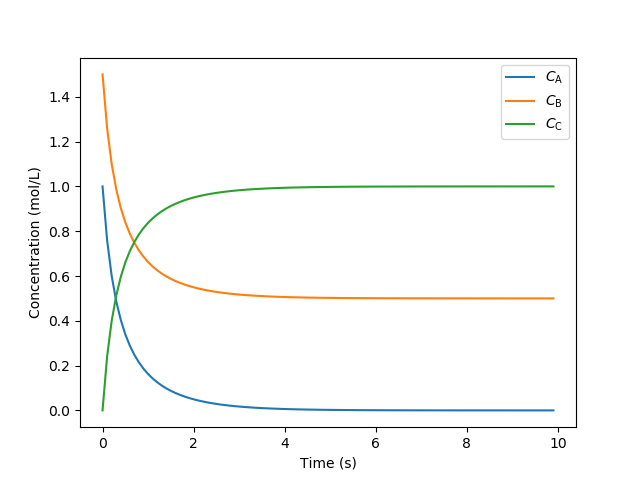
\includegraphics[width=.9\linewidth]{./conc.png}
\end{center}

\section{Lecture 4: Analyzing reactor data}
\label{sec:orge3dba3a}
\begin{enumerate}
\item Differential methods
\begin{enumerate}
\item Measuring rates
\end{enumerate}
\item Integral methods
\item Half-lives
\end{enumerate}


\begin{minted}[frame=lines,fontsize=\scriptsize,linenos]{python}
import numpy as np               #this lets up handles arrays of data
import matplotlib.pyplot as plt
from scipy.optimize import curve_fit

def differential(x, k, alpha):
    return k*x**alpha

def integral(t, a, b):
    return (2*a/(2+a*b*t))**2

t = np.array([0.00, 2.25, 4.50, 6.33, 8.00, 10.25, 12.00, 13.50, 15.60, 17.85, 19.60, 27.00, 30.00, 38.00, 41.00, 45.00, 47.00, 57.00, 63.00])

C_Br2 = np.array([0.3335, 0.2965, 0.2660, 0.2450, 0.2255, 0.2050, 0.1910, 0.1794, 0.1632, 0.1500, 0.1429, 0.1160, 0.1053, 0.0830, 0.0767, 0.0705, 0.0678, 0.0553, 0.0482])

plt.figure()
plt.plot(t,C_Br2,'o')
plt.xlabel('Time (s)')
plt.ylabel('Concentration (mol/L)')
plt.legend()
plt.savefig('./xylene-conc.png')

delta_t = np.ediff1d(t)        # finite difference between adjacent points
delta_C = np.ediff1d(C_Br2)

grad_t = np.gradient(t)            # second order approximation to gradient, allowing for unequal step size
grad_C = np.gradient(C_Br2)
rate = -np.divide(grad_C,grad_t)

plt.figure()
plt.plot(C_Br2,rate,'o')
plt.xlabel('Concentration (mol/L)')
plt.ylabel('Rate (mol/L/x)')
plt.legend()

popt, pcov = curve_fit(differential, C_Br2, rate )

print('k = {0:f}, alpha={1:f}'.format(popt[0],popt[1]))

model = differential(C_Br2,popt[0],popt[1])
plt.plot(C_Br2,model,'-')

plt.savefig('./xylene-rate.png')

difference_array = np. subtract(rate, model)
squared_array = np. square(difference_array)
mse = squared_array. mean()
print(mse)

# Suggests order of 1.5
popt1, pcov1 = curve_fit(integral, t, C_Br2)
print('k = {0:f}'.format(popt[1]))

model1 = integral(t, popt1[0], popt1[1])

plt.figure()
plt.plot(t,C_Br2,'o')
plt.plot(t,model1,'-')
plt.xlabel('Time (s)')
plt.ylabel('Concentration (mol/L)')
plt.legend()
plt.savefig('./xylene-int-model.png')


\end{minted}

\begin{verbatim}
k = 0.085277, alpha=1.450860
2.4942019231742367e-07
k = 1.450860
\end{verbatim}



\begin{center}
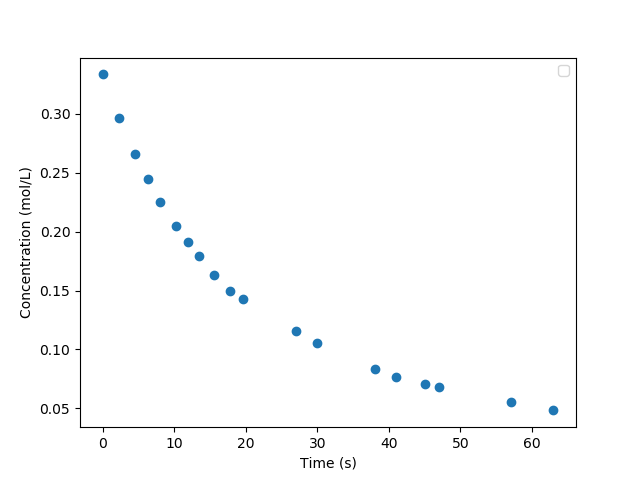
\includegraphics[width=.9\linewidth]{./xylene-conc.png}
\end{center}
\begin{center}
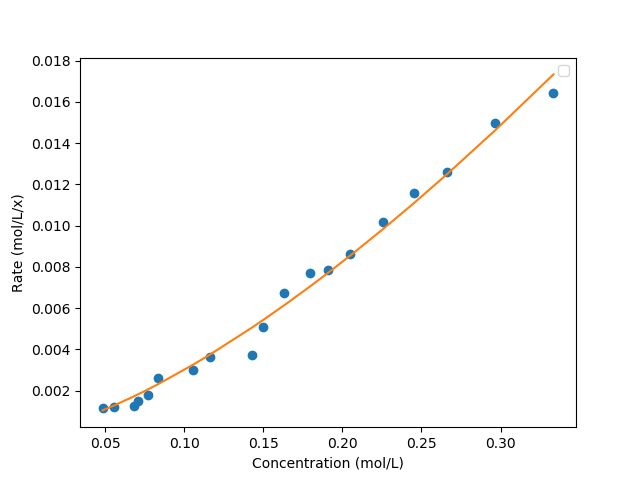
\includegraphics[width=.9\linewidth]{./xylene-rate.png}
\end{center}
\begin{center}
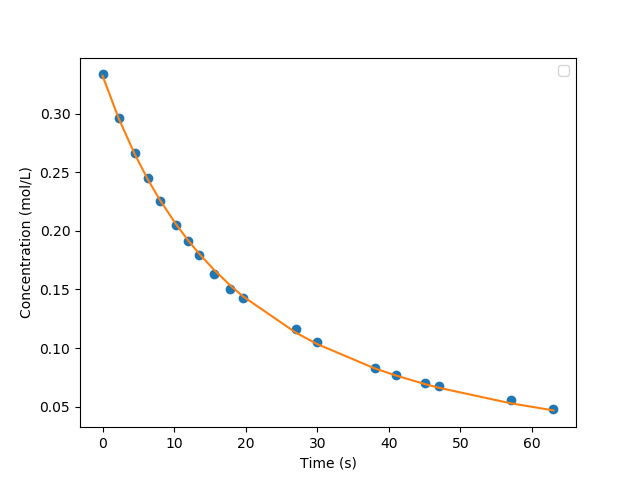
\includegraphics[width=.9\linewidth]{./xylene-int-model.png}
\end{center}

\section{Lecture 5: Molecular chemical kinetics}
\label{sec:orgab9dc76}
\subsubsection{Reaction mechanisms}
\label{sec:orgac3d1f0}
\begin{enumerate}
\item Elementary steps and molecularity
\item Ozone decomposition, rate second-order at high \(P_{\ce{O2}}\), first-order at low \(P_{\ce{O2}}\)
\begin{center}
\begin{tabular}{l}
\ce{2 O3 -> 3 O2}\\
\hline
\ce{O3 ->[k_1] O2 + O}\\
\ce{O2 + O ->[k_-1] O3}\\
\ce{O + O3 ->[k_2] 2 O2}\\
\end{tabular}
\end{center}
\item Detailed balance and microscopic reversibility
\item Equilibrium requirement \(K_{eq}(T) = k_f(T)/k_r(T)\)
\item Reversibility \(r_\text{net} = r_f ( 1 - \beta)\), \(\beta = Q/K_c = \exp(-\Delta G(T,c_j)/RT)\)
\begin{enumerate}
\item \ce{A <=> B} example
\end{enumerate}
\item Collision theory
\begin{enumerate}
\item A + B \(\rightarrow\) products
\item rate proportional to A/B collision frequency \(z_{AB}\) weighted by fraction of collisions with energy \(> E_a\)
\begin{displaymath}
   r = k C_A C_B , k = \left ( \frac{8 k_B T}{\pi \mu} \right )^{1/2} \sigma_{AB} N_{av} e^{-E_a/k_BT}
\end{displaymath}
\item upper bound on real rates
\end{enumerate}
\end{enumerate}
\subsubsection{Transition state theory (TST)}
\label{sec:orgceeb441}
\begin{enumerate}
\item Assumptions
\begin{enumerate}
\item Existence of reaction coordinate (PES)
\item Existence of dividing surface
\item Equilibrium between reactants and ``transition state''
\item Harmonic approximation for transition state
\end{enumerate}
\item rate proportional to concentration of ``activated complex'' over reactants times crossing frequency
\begin{eqnarray*}
   r & = & k C_AC_B \\
     & = & k^\ddagger C_{AB}^\ddagger \\
     & = & \nu^\ddagger K^\ddagger C_A C_ B \\
     & = & \nu^\ddagger \frac{k_BT}{h\nu^\ddagger}\bar{K}^\ddagger(T) C_A C_B \\
     & = & \frac{k_B T}{h} \frac{q^\ddagger(T)}{q_A(T) q_B(T)}  e^{-{\Delta E(0)/k_BT}} C_A C_B
\end{eqnarray*}
\end{enumerate}

\begin{center}
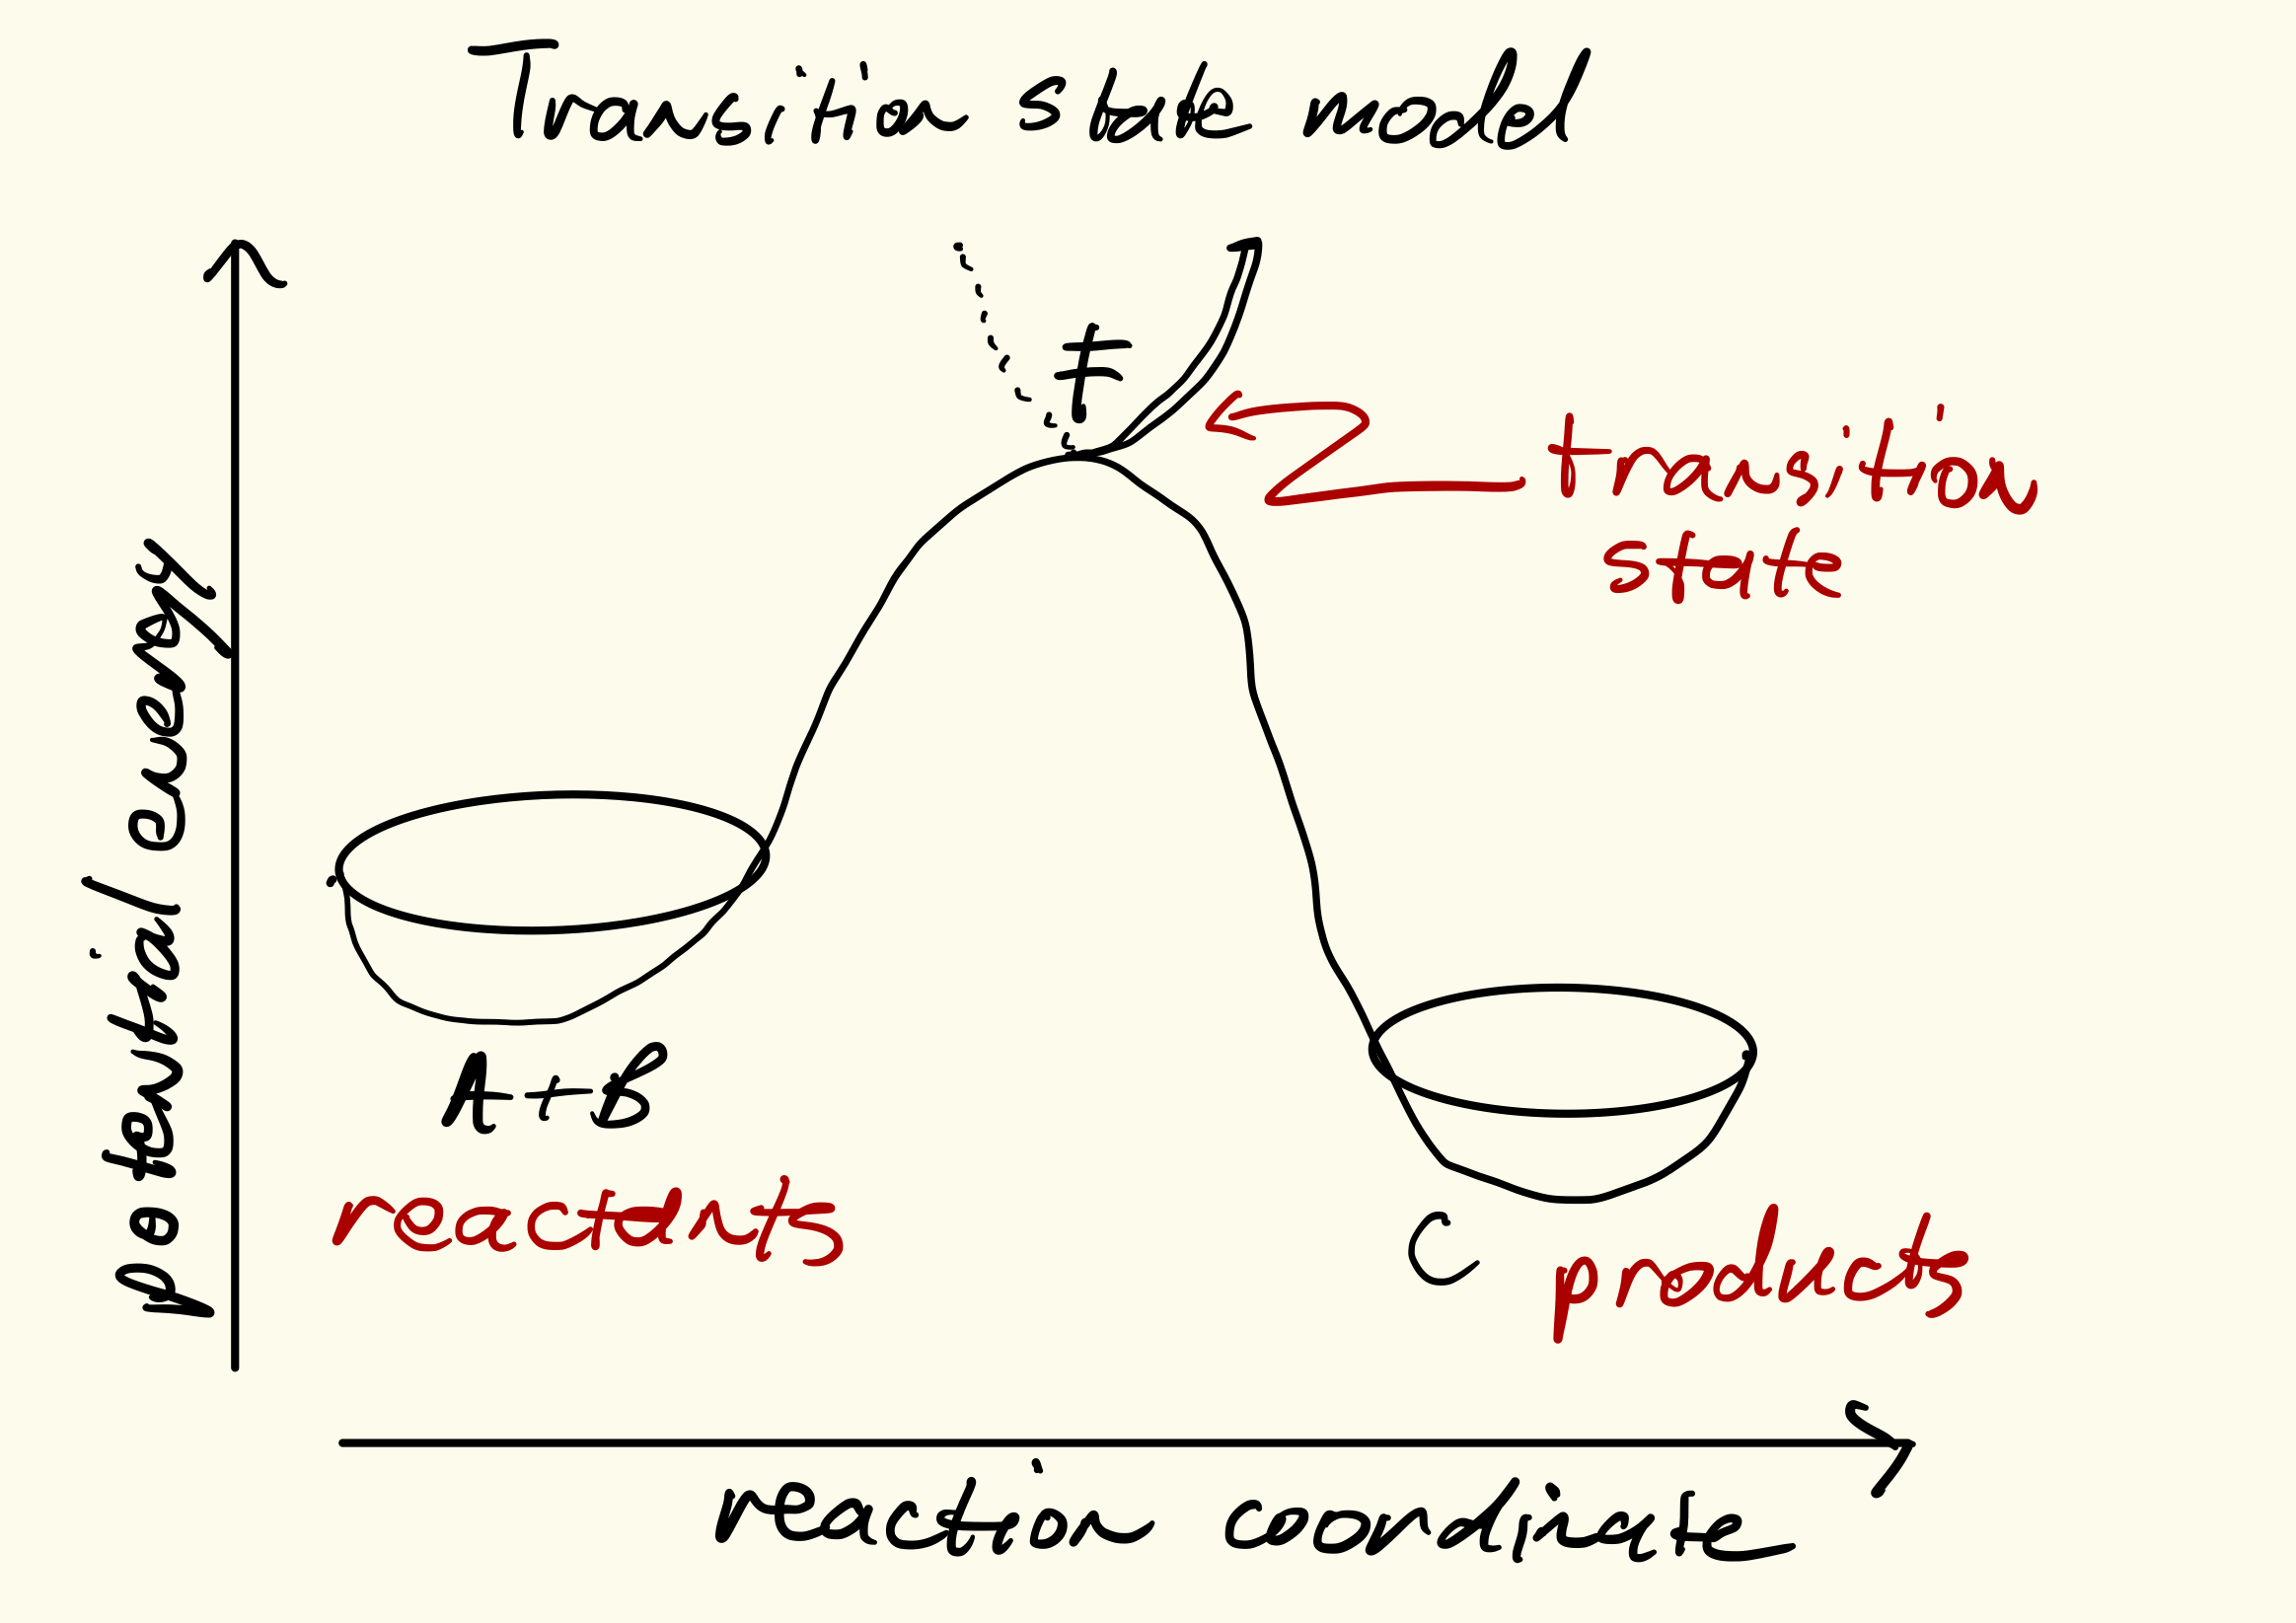
\includegraphics[width=0.6\textwidth]{./Images/PES.png}
\end{center}
\subsubsection{Locating transition states computationally}
\label{sec:orga182508}
\begin{enumerate}
\item Reactants/products are minima on potential energy surface
\item Transition state is first order saddle point. Unique point on pathway from reactant to product valley
\item vinyl alcohol to acetaldehyde example
\item \url{https://www.webmo.net}
\end{enumerate}

\begin{center}
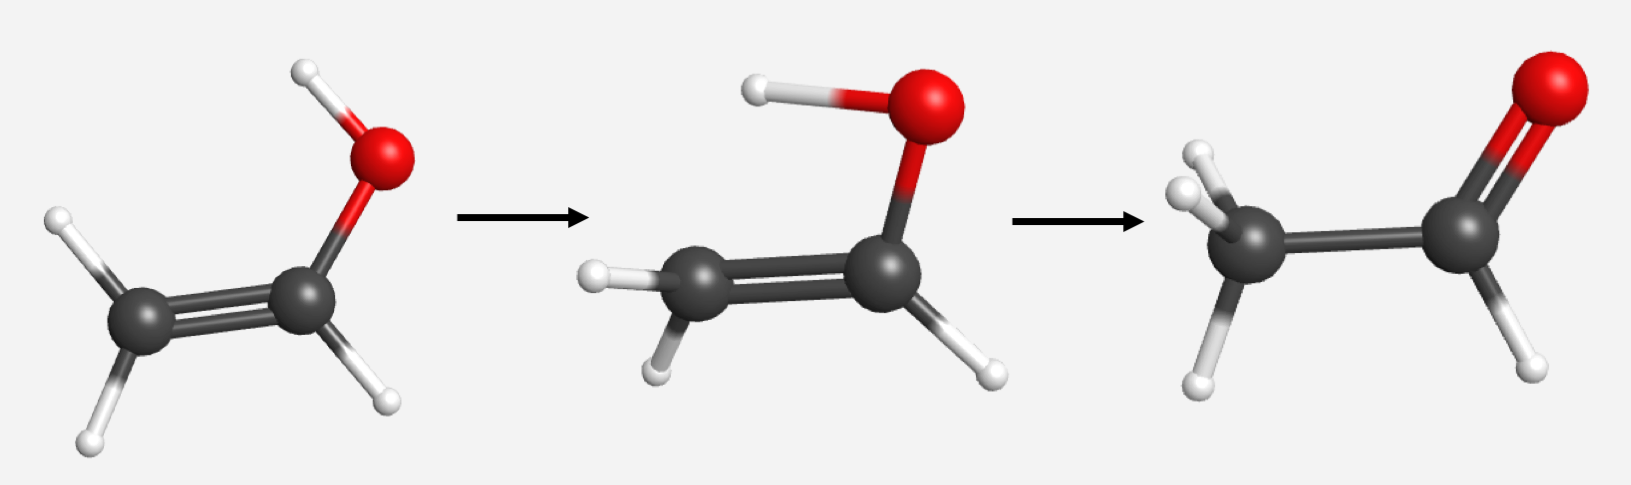
\includegraphics[width=.9\linewidth]{./Images/Path.png}
\end{center}

\subsubsection{Thermodynamic connection}
\label{sec:org9ee3df1}
\begin{enumerate}
\item Relate activated complex equilibrium constant to activation free energy (isochoric standard state)
\[ \(\bar{K}^\ddagger(T) = e^{-\Delta A^{\circ \ddagger}(T)/kT} = e^{-\Delta U^{\circ \ddagger}(T)/k_BT}e^{\Delta S^{\circ \ddagger}(T)/k_B} \]
\item Compare to Arrhenius expression 
\[E_a = \Delta U^{\circ \ddagger}(T) + kT, A = \frac{k_B T}{h}e^1e^{\Delta S^{\circ \ddagger}(T)/k_B}\]
\end{enumerate}

\begin{verbatim}
Vinyl alcohol to TS  216 kJ/mol
Delta Uddagger (1000 K) =  211 kJ/mol
Delta Addagger (1000 K) =  226 kJ/mol
Delta Sddagger (1000 K) = -1480 J/mol K
\end{verbatim}


\begin{center}
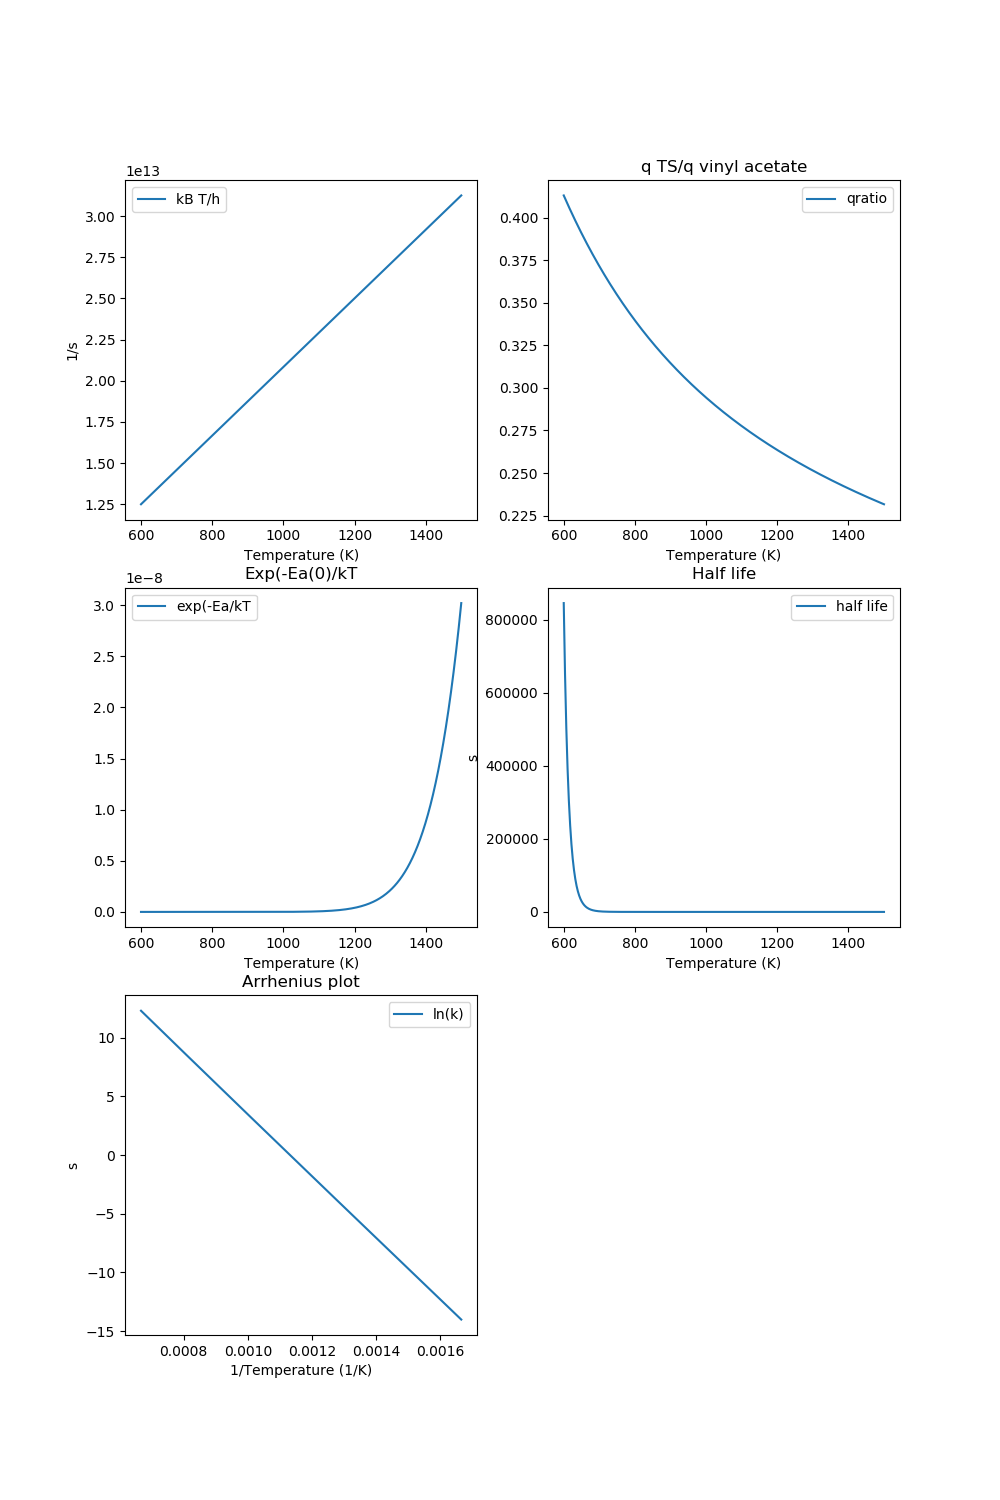
\includegraphics[width=.9\linewidth]{./Images/arrhenius.png}
\end{center}
\begin{center}
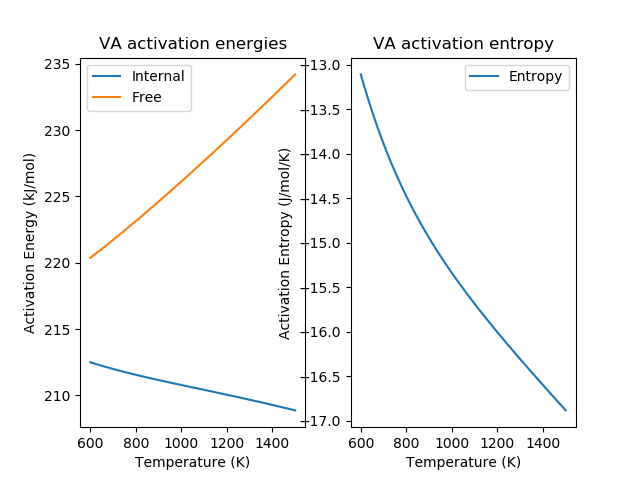
\includegraphics[width=.9\linewidth]{./Images/Sact.png}
\end{center}

\subsubsection{Bimolecular reaction}
\label{sec:orgbac67fa}
\begin{enumerate}
\item Diels-Alder example
\end{enumerate}

\begin{minted}[frame=lines,fontsize=\scriptsize,linenos]{python}
import numpy as np

kB = 8.61733e-5      # eV /K
h = 4.13566766e-15  # eV s
eVtokJ = 96.485332
Nav = 6.022e23      # Avogadro's number 
R0 = kB * eVtokJ * 1000.       # gas constant in J/mol K

A = 9.2e6 # liter/mole/second
Ea = 99. # kJ/mole

T = 500.   # K


# 1 M standard state
deltaUdd = Ea - R0 * T /1000   # kJ /mol

SS = 1.0  # mol/liter
deltaSdd = R0 * ( np.log(A/(1./SS)) - np.log(kB * T / h) - 1.)

deltaAdd = deltaUdd - T * deltaSdd/1000.

print('1 M standard state, 500 K:')
print('Delta Udd ={:4.0f} kJ/mol    Delta Sdd = {:4.0f} J/mol K   Delta Add = {:4.0f} kJ/mol'.format(deltaUdd,deltaSdd,deltaAdd))

# 1 bar standard state
P0 = 1.0e5   # 1 bar = 10^5 Pa = 10^5 J/m^3
P0 = P0 / 1e3  # J/l
SS = P0/(R0 * T)   #  J/mol / J/l  = mol/liter
print('1 bar = {:5.3f} mol/liter standard state, 500 K'.format(SS))

deltaHdd = Ea - 2* R0 * T /1000   # kJ /mol
deltaSdd = R0 * ( np.log(A/(1./SS)) - np.log(kB * T / h) - 2.)

deltaGdd = deltaHdd - T * deltaSdd/1000.
print('Delta Hdd ={:4.0f} kJ/mol    Delta Sdd = {:4.0f} J/mol K   Delta Gdd = {:4.0f} kJ/mol'.format(deltaHdd,deltaSdd,deltaGdd))

\end{minted}

\begin{verbatim}
1 M standard state, 500 K:
Delta Udd =  95 kJ/mol    Delta Sdd = -124 J/mol K   Delta Add =  157 kJ/mol
1 bar = 0.024 mol/liter standard state, 500 K
Delta Hdd =  91 kJ/mol    Delta Sdd = -164 J/mol K   Delta Gdd =  172 kJ/mol
\end{verbatim}

\subsubsection{Correlations across reactions}
\label{sec:org1b1affc}
\begin{enumerate}
\item early vs late transition states
\item Br\o{}nsted-Evans-Polyani relationship
\[ E_a = \alpha \Delta H + \beta \]
\item linear free energy relationships between similar reactions (substituent effects)
\[ \ln (k_1/k_1^\prime) \propto \ln (K_1/K_1^\prime) \]
\item compensation effect linear correlation across catalysts for the same reaction
\[\Delta H^{\circ\ddagger} \propto \Delta S^{\circ\ddagger}\]
\end{enumerate}
\section{Lecture 6: Reaction networks}
\label{sec:org880f7a1}

\subsection{Simple and visible}
\label{sec:org1915153}
\begin{enumerate}
\item Open vs closed (catalyzed) networks
\item \ce{A <-> B <-> C} reaction
\item free energy surface
\item Characterizations
\begin{enumerate}
\item instantaneous selectivity
\item overall selectivity
\item yield
\end{enumerate}
\item species rates vs reaction rates
\begin{enumerate}
\item Vector representations of rates
\end{enumerate}
\item Rate determining and degree of rate control
\item Equilibrium limited
\end{enumerate}

\begin{minted}[frame=lines,fontsize=\scriptsize,linenos]{python}
import numpy as np               #this lets up handles arrays of data
import matplotlib.pyplot as plt
from scipy.integrate import odeint, solve_ivp
from scipy.interpolate import BPoly

kB = 8.61733e-5      # eV /K
h = 4.13566766e-15  # eV s

def dCdt(C,t,k):
    dC_Adt = -k[0]*C[0]+k[1]*C[1]     # A <->  B <-> C;  r = k CA CB
    dC_Bdt =  k[0]*C[0]-k[1]*C[1] -k[2]*C[1]+k[3]*C[2]
    dC_Cdt =  k[2]*C[1]-k[3]*C[2]
    dCdt = [dC_Adt,dC_Bdt,dC_Cdt] 
    return dCdt

# initialize concentrations
C_0 = [1., 0, 0.]

R0 = 8.314
T = 500.

# initialize k's
deltaGtot = -100.0; deltaG1 = -50.0; deltaG1d = 125. ; deltaG2d = 125.

deltaG2 = deltaGtot - deltaG1
deltaGn1d = deltaG1d-deltaG1
deltaGn2d = deltaG2d-deltaG2

p1 = BPoly.from_derivatives([0, 1, 2, 3, 4], [[0, 0], [deltaG1d, 0], [deltaG1, 0], [deltaG1+deltaG2d,0], [deltaGtot,0]])

x=np.linspace(0,4,100)
y=p1(x)

plt.figure(figsize=(10,12))
plt.subplot(2,2,1)
plt.plot(x,y)
plt.ylabel('Free energy')
plt.xlabel('Reaction coordinate')

k = (kB*T/h)*np.exp(-np.array([deltaG1d,deltaGn1d,deltaG2d,deltaGn2d])*1000./(R0*T))
print('T = {:4.1f}'.format(T))
print('Delta G1 = {:4.1f}  deltaG1dagger = {:4.1f}  delta G2 = {:4.1f}   deltaG2d = {:4.1f} kJ/mol'.format(deltaG1,deltaG1d,deltaG2,deltaG2d))
print('k1 = {:6.3e}     k-1 = {:6.3e}         k2 = {:6.3e}      k-2 = {:6.3e} /s'.format(k[0],k[1],k[2],k[3]))

# Range of time to solve over
t = np.arange(0,6,0.1) 

p = (k,) # turn parameters into a tuple
C = odeint(dCdt,C_0,t,p)
C_A = C.transpose()[0] # Get C_A from C
C_B = C.transpose()[1] # Get C_B from C
C_C = C.transpose()[2]

plt.subplot(2,2,2)
plt.plot(t,C_A,'-',label=r'$C_{\rm A}$')
plt.plot(t,C_B,'-',label=r'$C_{\rm B}$')
plt.plot(t,C_C,'-',label=r'$C_{\rm C}$')
plt.xlabel('Time (s)')
plt.ylabel('Concentration (mol/L)')
plt.legend()

plt.subplot(2,2,3)
plt.plot(t,-k[0]*C_A+k[1]*C_B,label=r'$r_{\rm A}$')
plt.plot(t,k[0]*C_A-k[1]*C_B-k[2]*C_B + k[3]*C_C,label=r'$r_{\rm B}$')
plt.plot(t,k[2]*C_B-k[3]*C_C,label=r'$r_{\rm C}$')
plt.xlabel('Time (s)')
plt.ylabel('Rate (mol/L/s)')
plt.title('Species rates')
plt.legend()

plt.subplot(2,2,4)
plt.plot(t,k[0]*C_A,label=r'$r_1$')
plt.plot(t,k[1]*C_B,label=r'$r_{-1}$')
plt.plot(t,k[2]*C_B,label=r'$r_2$')
plt.plot(t,k[3]*C_C,label=r'$r_{-2}$')
plt.xlabel('Time (s)')
plt.ylabel('Rate (mol/L/s)')
plt.title('Reaction rates')
plt.legend()

plt.savefig('./Images/ABC-rxn.png')
\end{minted}

\begin{verbatim}
T = 500.0
Delta G1 = -50.0  deltaG1dagger = 125.0  delta G2 = -50.0   deltaG2d = 125.0 kJ/mol
k1 = 9.092e-01     k-1 = 5.433e-06         k2 = 9.092e-01      k-2 = 5.433e-06 /s
\end{verbatim}


\begin{center}
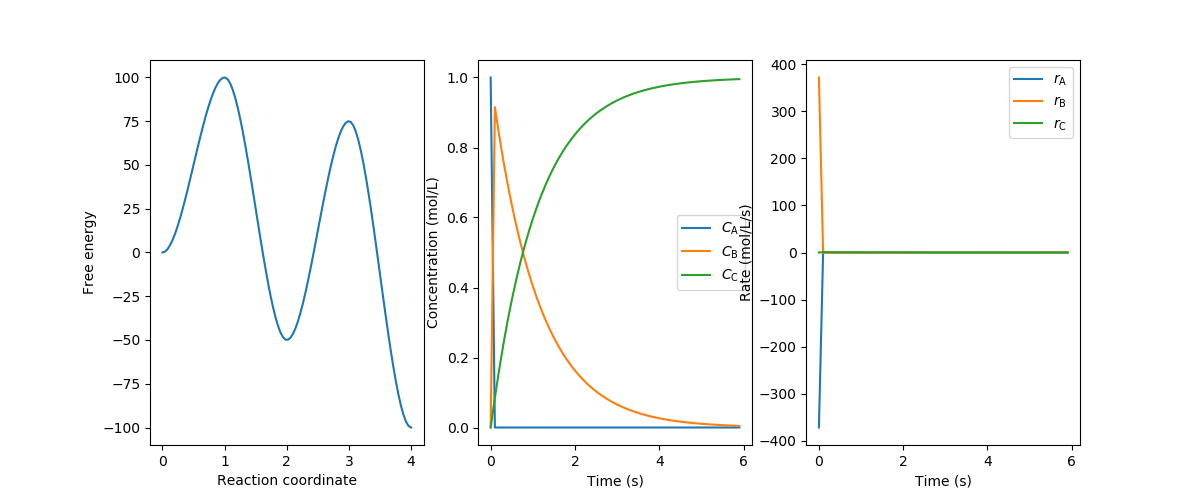
\includegraphics[width=.9\linewidth]{./Images/ABC-rxn.png}
\end{center}
\subsection{Simply and invisible}
\label{sec:org4399ce3}
\begin{enumerate}
\item Lindemann-Hinshelwood model for first order reactions
\item Irreversible steps
\item Pseudo-steady state approximation
\begin{enumerate}
\item \ce{A -> B -> C} in limit \(k_2 > k_1\)
\end{enumerate}
\[ r_{\text{B}} \approx 0 \]     \[C_\text{B,max} \approx 0 \]
  \[C_A = C_{A0} e^{-k_1 t}\]    \[C_B= C_{A0}\frac{k_1}{k_2-k_1} \left ( e^{-k_1 t} - e^{-k_2 t} \right ) \]
\begin{enumerate}
\item B intermediate \(\rightarrow\) reactive intermediate
\end{enumerate}
\end{enumerate}


\begin{verbatim}
T = 500.0
Delta G1 = -50.0  deltaG1dagger = 125.0  delta G2 = -50.0   deltaG2d = 100.0 kJ/mol
k1 = 9.092e-01     k-1 = 5.433e-06         k2 = 3.720e+02      k-2 = 2.222e-03 /s
\end{verbatim}


\begin{center}
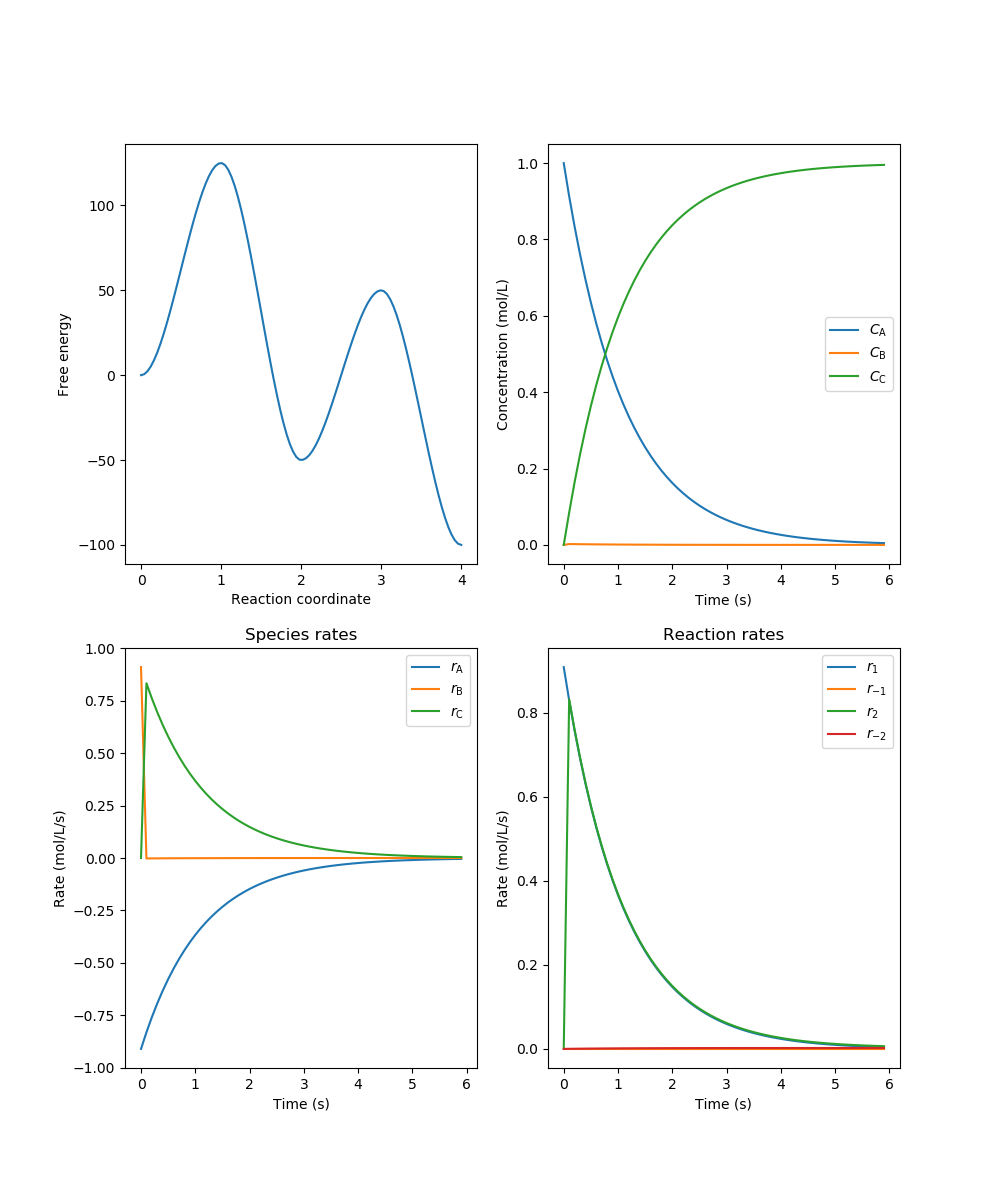
\includegraphics[width=.9\linewidth]{./Images/ABC-PSSA.png}
\end{center}


\subsection{Simplifying reaction networks}
\label{sec:org1f2adf1}
\begin{enumerate}
\item Simplifications helpful when parameters of full model are unknown or to fit to experimental observations
\item Ozone decomposition, \ce{2 O3 -> 3 O2} 
\[ \ce{O3 <=> O2 + O} \]
\[ \ce{O + O3 -> 2 O2} \]
\begin{enumerate}
\item PSSA
\[ -r_{O3} = \frac{2 k_1 k_2 C^2_{\ce{O3}}}{k_{-1} C_{\ce{O2}} + k_2 C_{\ce{O3}}} \]
\item Limiting behaviors
\end{enumerate}
\item CO chlorination (closed)
\[ \ce{Cl2 <=>[h\nu] 2 Cl*}\]
\[ \ce{CO + Cl* <=> COCl*} \]
\[ \ce{COCl* + Cl2 <=> COCl2 + Cl*} \]
\item Ethane pyrolysis \ce{C2H6 -> C2H4 + H2} (open)
\end{enumerate}
\begin{center}
\begin{tabular}{llr}
\hline
 & \(A\) (\si{\per\second}) & \(E_a\) (\si{\kilo\joule\per\mole})\\
\hline
\ce{C2H6 -> 2 CH3} & \SI{1.0e17}{} & 356\\
\ce{CH3 + C2H6 -> CH4 + C2H5 } & \SI{2.0e11}{} & 44\\
\ce{C2H5 -> C2H4 + H } & \SI{3.0e14}{} & 165\\
\ce{H + C2H6 -> H2 + C2H5} & \SI{3.4e12}{} & 28\\
\ce{H + C2H5 -> C2H6} & \SI{1.6e13}{} & 0\\
\hline
\end{tabular}
\end{center}
\begin{enumerate}
\item Chain reactions
\begin{enumerate}
\item Polymerization
\end{enumerate}
\end{enumerate}

\subsection{Complex reaction networks}
\label{sec:org8197ee5}
\begin{enumerate}
\item Ethane pyrolysis redux,  \href{https://pubs.acs.org/doi/10.1021/jp206503d}{doi:10.1021/jp206503d}
\end{enumerate}

\subsection{Stochastic solutions}
\label{sec:org599013a}

\begin{minted}[frame=lines,fontsize=\scriptsize,linenos]{python}
import numpy as np
import matplotlib.pyplot as plt 
from scipy.integrate import odeint, solve_ivp

Nav = 6.022e23
l_to_nm3 = 1e21

def dCdt(C,t,k):
    dC_Adt = -k[0]*C[0]     # A ->  B -> C;  r = k CA CB
    dC_Bdt = k[0]*C[0]-k[1]*C[1]
    dC_Cdt =  k[1]*C[1]
    dCdt = [dC_Adt,dC_Bdt,dC_Cdt] 
    return dCdt

Ntot = 75  # set total number of particles

CA0 = 1.0  # set initial concentrations, mol/l
CB0 = 0.0
CC0 = 0.0

k = np.array([1.0,1.0])   # /second

Ctot = CA0 + CB0 + CC0

Volume = Ntot/Ctot # number/mol/liter
side = Volume**(1/3)

na = Ntot *(CA0/Ctot); nb = Ntot *(CB0/Ctot); nc = Ntot *(CC0/Ctot); tnow = 0.

NA = np.array([na])
NB = np.array([nb])
NC = np.array([nc])
t = np.array([tnow])

while na > 0 or nb > 0:  # While there is still A and B left, there will be reaction occurring.
    p1 = np.random.random_sample()  # Get random number from 0 to 1.
    p2 = np.random.random_sample()
    r1 = k[0] * na  # Definition for the reaction mechanism.
    r2 = k[1] * nb
    if p2 < (r1/(r1+r2)):  # Monte Carlo step
        na-=1;  nb+=1
    else:
        nb-=1;  nc+=1

    dt = -np.log(p1) / (r1 + r2)  # This is the time interval until the next reaction to occur.
    tnow+= dt  # To refresh the time for next circulation.
    
    NA = np.append(NA,na)  # inelegant and wasteful
    NB = np.append(NB,nb)
    NC = np.append(NC,nc)
    t  = np.append(t,tnow)

#    open('KMC_data.txt','w+').write('\n'.join('%f, %i, %i, %i' %x for x in data))
    # Record data of this circulation to the .txt file.

# analytical solution
C_0 = [CA0, CB0, CC0]
ta = np.arange(0,10,0.1) 
p = (k,) # turn parameters into a tuple
C = odeint(dCdt,C_0,ta,p)

C_A = C.transpose()[0] # Get C_A from C
C_B = C.transpose()[1] # Get C_B from C
C_C = C.transpose()[2]

# Plot with the data acquired above.
plt.figure()
plt.plot(t, NA, 'o', markersize = '3', label=r'$N_{\rm A}$')  # Configure for the first line.
plt.plot(t, NB, 'o', markersize = '3', label=r'$N_{\rm B}$')
plt.plot(t, NC, 'o', markersize = '3', label=r'$N_{\rm C}$')
plt.plot(ta,C_A*Volume,'-',color='blue')
plt.plot(ta,C_B*Volume,'-',color='orange')
plt.plot(ta,C_C*Volume,'-',color='green')
plt.legend()
plt.title('Stochastic vs analytical evolution of A->B->C')
plt.xlabel('time (s)')  # Labeling the axis.
plt.ylabel('Molecules')
plt.savefig('./Images/kMC.png')
\end{minted}

\begin{center}
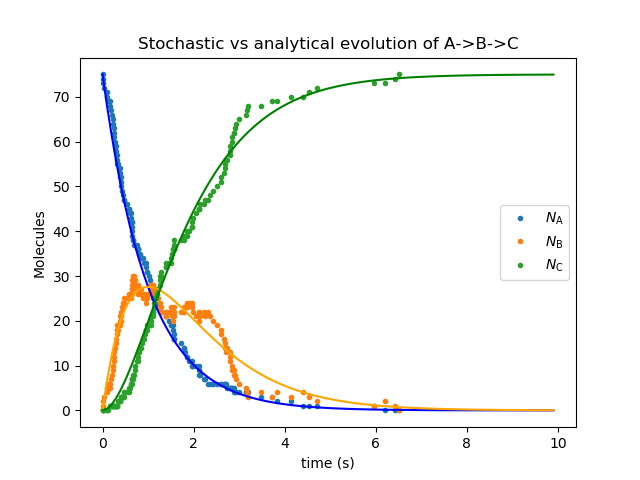
\includegraphics[width=.9\linewidth]{./Images/kMC.png}
\end{center}




\section{Heterogeneous reactions}
\label{sec:org1217c51}
\begin{enumerate}
\item adsorption, L-H
\item TPD
\item catalysis
\item Sabatier analysis
\end{enumerate}
\subsubsection{Heterogeneous reactions and catalysis}
\label{sec:orge7e8ec1}
\begin{enumerate}
\item molecule-surface collisions
\item surface reactions
\item Ammonia oxidation, \ce{NH3 + O2 -> NO + N2}, \href{http://pubs.acs.org/doi/10.1021/acscatal.8b04251}{doi:10.1021/acscatal.8b04251}
\end{enumerate}

\section{Liquid-phase reactions}
\label{sec:org8ba2ad2}
\subsubsection{Diffusion-controlled reactions}
\label{sec:org219101c}
\begin{enumerate}
\item Intermediate complex
\item Steady-state approximation
\item Diffusion-controlled limit (\(k_D = 4\pi (r_A + r_B) D_{AB}\))
\item Reaction-controlled limit (\(k_{app}=(k_D/k_{-D})k_r\))
\end{enumerate}

\begin{table}
\begin{center}
    \caption{\large{Equilibrium and Rate Constants}}
   \begin{description}
   \item[Equilibrium Constants] $a~\text{A} + b~\text{B} \rightleftharpoons c~\text{C} + d~\text{D} $
     \begin{eqnarray*}
       K_{eq}(T) &=& e^{\Delta S^\circ(T)/k_B}e^{-\Delta H^\circ(T)/k_BT}
       \\ \\
            K_c(T) &=&
          \left(\frac{1}{c^\circ}\right)^{\nu_c+\nu_d-\nu_a-\nu_b}\frac{(q_c/V)^{\nu_c}(q_d/V)^{\nu_d}}{(q_a/V)^{\nu_a}(q_b/V)^{\nu_b}}e^{-\Delta
            E(0)\beta}\\ \\
            K_p(T) &=&
          \left(\frac{k_BT}{P^\circ}\right)^{\nu_c+\nu_d-\nu_a-\nu_b}\frac{(q_c/V)^{\nu_c}(q_d/V)^{\nu_d}}{(q_a/V)^{\nu_a}(q_b/V)^{\nu_b}}e^{-\Delta
            E(0)\beta}
\end{eqnarray*}
\item[Unimolecular Reaction] $\text[A] \rightleftharpoons [\text{A} ]^\ddagger
  \rightarrow C$
      \begin{displaymath}
        k(T)=\nu^\ddagger \bar K^\ddagger=\frac{k_B T}{h} \frac{\bar{q}_\ddagger(T)/V}{q_A(T)/V}
          e^{-\Delta E^\ddagger(0)\beta}
      \end{displaymath}
\begin{center}
      \begin{tabular}{cc}
      $ \displaystyle E_a =\Delta H^{\circ\ddagger}+k_B T $
      & $ \displaystyle A = e^1\frac{k_B T}{h} e^{\Delta S^{\circ\ddagger}} $
      \end{tabular}
\end{center}
\item[Bimolecular Reaction] $
        \mathrm{A} + \mathrm{B} \rightleftharpoons [ \mathrm{AB}]^\ddagger
        \rightarrow \text{C}$
      \begin{displaymath}
        k(T)=\nu^\ddagger \bar K^\ddagger=\frac{k_B T}{h} \frac{q_\ddagger(T)/V}{(q_A(T)/V)(q_B(T)/V)}\left
          (\frac{1}{c^\circ}\right )^{-1}
        e^{-\Delta E^\ddagger(0)\beta}
      \end{displaymath}
      \begin{center}
        \begin{tabular}{cc}
        $ \displaystyle E_a  =\Delta H^{\circ\ddagger}+2 k_B T $ & $ \displaystyle
        A  = e^2\frac{k_B T}{h} e^{\Delta S^{\circ\ddagger}} $
      \end{tabular}
      \end{center}
   \end{description}
 \end{center}
 \end{table}
\end{document}